%% LyX 2.2.2 created this file.  For more info, see http://www.lyx.org/.
%% Do not edit unless you really know what you are doing.
\documentclass[ruled]{article}
\usepackage{courier}
\usepackage[latin9]{inputenc}
\usepackage[letterpaper]{geometry}
\geometry{verbose}
\usepackage{color}
\usepackage{url}
\usepackage{algorithm2e}
\usepackage{amsmath}
\usepackage[unicode=true,
 bookmarks=false,
 breaklinks=false,pdfborder={0 0 1},backref=section,colorlinks=true]
 {hyperref}
\usepackage{graphicx}

\makeatletter

%%%%%%%%%%%%%%%%%%%%%%%%%%%%%% LyX specific LaTeX commands.
\providecommand{\LyX}{\texorpdfstring%
  {L\kern-.1667em\lower.25em\hbox{Y}\kern-.125emX\@}
  {LyX}}

%%%%%%%%%%%%%%%%%%%%%%%%%%%%%% User specified LaTeX commands.
\title{Machine Learning and Computational Statistics, Spring 2016\\
Homework 1: Ridge Regression and SGD\\
Yidi Zhang} 
\date{}
%\date{February $4^{th}$, 6pm}




\usepackage{amsfonts}\usepackage{capt-of}
%\usepackage{url}
\usepackage{graphicx}
\usepackage{color}
\usepackage{bbm}
\usepackage{enumerate}
\newcommand{\carlos}[1]{\textcolor{red}{Carlos: #1}}
\newcommand{\field}[1]{\mathbb{#1}} 
\newcommand{\hide}[1]{#1}
\newcommand{\pd}[2]{\frac{\partial #1}{\partial #2}}
\providecommand{\m}[1]{\mathbf{#1}}
\providecommand{\norm}[1]{\left\|#1\right\|}
\providecommand{\sign}[1]{\text{sign}\left(#1\right)}
\DeclareMathOperator*{\argmin}{arg\,min}
\providecommand{\what}{\m{\hat{w}}}
\providecommand{\dw}{\Delta w}
\providecommand{\dmw}{\Delta \m{w}}
\providecommand{\hy}{\hat{y}}

\usepackage{listings}
\usepackage{color}

\definecolor{dkgreen}{rgb}{0,0.6,0}
\definecolor{gray}{rgb}{0.5,0.5,0.5}
\definecolor{mauve}{rgb}{0.58,0,0.82}

\lstset{frame=tb,
  language=Java,
  aboveskip=3mm,
  belowskip=3mm,
  showstringspaces=false,
  columns=flexible,
  basicstyle={\small\ttfamily},
  numbers=none,
  numberstyle=\tiny\color{gray},
  keywordstyle=\color{blue},
  commentstyle=\color{dkgreen},
  stringstyle=\color{mauve},
  breaklines=true,
  breakatwhitespace=true,
  tabsize=3
}

\makeatother

\begin{document}
\global\long\def\reals{\mathbf{R}}
 \global\long\def\integers{\mathbf{Z}}
\global\long\def\naturals{\mathbf{N}}
 \global\long\def\rationals{\mathbf{Q}}
\global\long\def\ca{\mathcal{A}}
\global\long\def\cb{\mathcal{B}}
 \global\long\def\cc{\mathcal{C}}
 \global\long\def\cd{\mathcal{D}}
\global\long\def\ce{\mathcal{E}}
\global\long\def\cf{\mathcal{F}}
\global\long\def\cg{\mathcal{G}}
\global\long\def\ch{\mathcal{H}}
\global\long\def\ci{\mathcal{I}}
\global\long\def\cj{\mathcal{J}}
\global\long\def\ck{\mathcal{K}}
\global\long\def\cl{\mathcal{L}}
\global\long\def\cm{\mathcal{M}}
\global\long\def\cn{\mathcal{N}}
\global\long\def\co{\mathcal{O}}
\global\long\def\cp{\mathcal{P}}
\global\long\def\cq{\mathcal{Q}}
\global\long\def\calr{\mathcal{R}}
\global\long\def\cs{\mathcal{S}}
\global\long\def\ct{\mathcal{T}}
\global\long\def\cu{\mathcal{U}}
\global\long\def\cv{\mathcal{V}}
\global\long\def\cw{\mathcal{W}}
\global\long\def\cx{\mathcal{X}}
\global\long\def\cy{\mathcal{Y}}
\global\long\def\cz{\mathcal{Z}}
\global\long\def\ind#1{1(#1)}
\global\long\def\pr{\mathbb{P}}
\global\long\def\predsp{\cy}
\global\long\def\outsp{\cy}
\global\long\def\prxy{P_{\cx\times\cy}}
\global\long\def\prx{P_{\cx}}
\global\long\def\prygivenx{P_{\cy\mid\cx}}
\global\long\def\ex{\mathbb{E}}
\global\long\def\var{\textrm{Var}}
\global\long\def\cov{\textrm{Cov}}
\global\long\def\sgn{\textrm{sgn}}
\global\long\def\sign{\textrm{sign}}
\global\long\def\kl{\textrm{KL}}
\global\long\def\law{\mathcal{L}}
\global\long\def\eps{\varepsilon}
\global\long\def\as{\textrm{ a.s.}}
\global\long\def\io{\textrm{ i.o.}}
\global\long\def\ev{\textrm{ ev.}}
\global\long\def\convd{\stackrel{d}{\to}}
\global\long\def\eqd{\stackrel{d}{=}}
\global\long\def\del{\nabla}
\global\long\def\loss{\ell}
\global\long\def\risk{R}
\global\long\def\emprisk{\hat{R}_{\ell}}
\global\long\def\lossfnl{L}
\global\long\def\emplossfnl{\hat{L}}
\global\long\def\empminimizer#1{\hat{#1}_{\ell}}
\global\long\def\minimizer#1{#1_{*}}
\global\long\def\etal{\textrm{et. al.}}
\global\long\def\tr{\operatorname{tr}}
\global\long\def\trace{\operatorname{trace}}
\global\long\def\diag{\text{diag}}
\global\long\def\rank{\text{rank}}
\global\long\def\linspan{\text{span}}
\global\long\def\proj{\text{Proj}}
\global\long\def\argmax{\operatornamewithlimits{arg\, max}}
\global\long\def\argmin{\operatornamewithlimits{arg\, min}}
\global\long\def\bfx{\mathbf{x}}
\global\long\def\bfy{\mathbf{y}}
\global\long\def\bfl{\mathbf{\lambda}}
\global\long\def\bfm{\mathbf{\mu}}
\global\long\def\calL{\mathcal{L}}
\global\long\def\vw{\boldsymbol{w}}
\global\long\def\vx{\boldsymbol{x}}
\global\long\def\vxi{\boldsymbol{\xi}}
\global\long\def\valpha{\boldsymbol{\alpha}}
\global\long\def\vbeta{\boldsymbol{\beta}}
\global\long\def\vsigma{\boldsymbol{\sigma}}
\global\long\def\vmu{\boldsymbol{\mu}}
\global\long\def\vtheta{\boldsymbol{\theta}}
\global\long\def\vd{\boldsymbol{d}}
\global\long\def\vs{\boldsymbol{s}}
\global\long\def\vt{\boldsymbol{t}}
\global\long\def\vh{\boldsymbol{h}}
\global\long\def\ve{\boldsymbol{e}}
\global\long\def\vf{\boldsymbol{f}}
\global\long\def\vg{\boldsymbol{g}}
\global\long\def\vz{\boldsymbol{z}}
\global\long\def\vk{\boldsymbol{k}}
\global\long\def\va{\boldsymbol{a}}
\global\long\def\vb{\boldsymbol{b}}
\global\long\def\vv{\boldsymbol{v}}
\global\long\def\vy{\boldsymbol{y}}
\global\long\def\hil{\ch}
\global\long\def\rkhs{\hil}
\maketitle

\textbf{Saturday, February 4, 2017}

\section{Introduction}

In this homework you will implement ridge regression using gradient
descent and stochastic gradient descent. We've provided a lot of support
Python code to get you started on the right track. References below
to particular functions that you should modify are referring to the
support code, which you can download from the website. If you have
time after completing the assignment, you might pursue some of the
following:
\begin{itemize}
\item Study up on numpy's \href{https://docs.scipy.org/doc/numpy/user/basics.broadcasting.html}{broadcasting}
to see if you can simplify and/or speed up your code.
\item Think about how you could make the code more modular so that you could
easily try different loss functions and step size methods. 
\item Experiment with more sophisticated approaches to setting the step
sizes for SGD (e.g. try out the recommendations in ``Bottou's SGD
Tricks'' on the website) 
\item Instead of taking 1 data point at a time, as in SGD, try minibatch
gradient descent, where you use multiple points at a time to get your
step direction. How does this effect convergence speed? Are you getting
computational speedup as well by using vectorized code?
\item Advanced: What kind of loss function will give us ``quantile regression''?
\end{itemize}
I encourage you to develop the habit of asking ``what if?'' questions
and then seeking the answers. I guarantee this will give you a much
deeper understanding of the material (and likely better performance
on the exam and job interviews, if that's your focus). You're also
encouraged to post your interesting questions on Piazza under ``questions'',
or on CrossValidated (\url{http://stats.stackexchange.com/}).

\section{Linear Regression}

\subsection{Feature Normalization}

When feature values differ greatly, we can get much slower rates of
convergence of gradient-based algorithms. Furthermore, when we start
using regularization (introduced in a later problem), features with
larger values can have a much greater effect on the final output for
the same regularization cost \textendash{} in effect, features with
larger values become more important once we start regularizing. One
common approach to feature normalization is to linearly transform
(i.e. shift and rescale) each feature so that all feature values in
the training set are in $[0,1]$. Each feature gets its own transformation.
We then apply the same transformations to each feature on the test\footnote{Throughout this assignment we refer to the ``test'' set. It may
be more appropriate to call this set the ``validation'' set, as
it will be a set of data on which compare the performance of multiple
models. Typically a test set is only used once, to assess the performance
of the model that performed best on the validation set.} set. It's important that the transformation is ``learned'' on the
training set, and then applied to the test set. It is possible that
some transformed test set values will lie outside the $[0,1]$ interval.

Modify function \texttt{feature\_normalization} to normalize all the
features to $[0,1]$. (Can you use numpy's ``broadcasting'' here?)

{\bfseries Answer 2.1:}

\begin{lstlisting}
def feature_normalization(train, test):
    """Rescale the data so that each feature in the training set is in
    the interval [0,1], and apply the same transformations to the test
    set, using the statistics computed on the training set.

    Args:
        train - training set, a 2D numpy array of size (num_instances, num_features)
        test  - test set, a 2D numpy array of size (num_instances, num_features)
    Returns:
        train_normalized - training set after normalization
        test_normalized  - test set after normalization

    """
    mins_train = np.min(train, axis=0)
    maxs_train = np.max(train, axis=0)
    rng_train = maxs_train - mins_train
    train_normalized = (train-mins_train)/rng_train
    
    mins_test = np.min(test, axis=0)
    maxs_test = np.max(test, axis=0)
    rng_test = maxs_test - mins_test
    test_normalized = (test-mins_test)/rng_test
    return train_normalized, test_normalized
    \end{lstlisting}

\subsection{Gradient Descent Setup} %%2.2

In linear regression, we consider the hypothesis space of linear functions
$h_{\theta}:\reals^{d}\to\reals$, where
\[
h_{\theta}(x)=\theta^{T}x,
\]
for $\theta,x\in\reals^{d}$, and we choose $\theta$ that minimizes
the following ``square loss'' objective function: 
\[
J(\theta)=\frac{1}{2m}\sum_{i=1}^{m}\left(h_{\theta}(x_{i})-y_{i}\right)^{2},
\]
where $(x_{1},y_{1}),\ldots,(x_{m},y_{m})\in\reals^{d}\times\reals$
is our training data.

While this formulation of linear regression is very convenient, it's
more standard to use a hypothesis space of ``affine'' functions:
\[
h_{\theta,b}(x)=\theta^{T}x+b,
\]
which allows a ``bias'' or nonzero intercept term. The standard
way to achieve this, while still maintaining the convenience of the
first representation, is to add an extra dimension to $x$ that is
always a fixed value, such as 1. You should convince yourself that
this is equivalent. We'll assume this representation, and thus we'll
actually take $\theta,x\in\reals^{d+1}$.
\begin{enumerate}
\item Let $X\in\reals^{m\times\left(d+1\right)}$ be the \textbf{design
matrix}, where the $i$'th row of $X$ is $x_{i}$. Let $y=\left(y_{1},\ldots,y_{m}\right)^{T}\in\reals^{m\times1}$
be a the ``response''. Write the objective function $J(\theta)$
as a matrix/vector expression, without using an explicit summation
sign.%%2.2.1

{\bfseries 2.2.1 Answer:}
The vector expression of objective function $J(\theta)$ is:
$$J(\theta)=\frac{1}{2m}(X\theta-y)^{T}(X\theta-y)=\frac{1}{2m}||X\theta-y||^{2}_{2}$$
 

\item Write down an expression for the gradient of $J$. %%2.2.2

{\bfseries 2.2.2 Answer:}
The expression for the gradient of $J$ is:
$$\del_{\theta}J(\theta)=\frac{1}{m}X^{T}(X\theta-y)$$

\item In our search for a $\theta$ that minimizes $J$, suppose we take%%2.2.3
a step from $\theta$ to $\theta+\eta\Delta$, where $\Delta\in\reals^{d+1}$
is a unit vector giving the direction of the step, and $\eta\in\reals$
is the length of the step. Use the gradient to write down an approximate
expression for $J(\theta+\eta\Delta)-J(\theta)$. {[}This approximation
is called a ``linear'' or ``first-order'' approximation.{]}

{\bfseries 2.2.3 Answer:}
The approximate expression for $J(\theta+\eta\Delta)-J(\theta)$ is:
$$J(\theta+\eta\Delta)-J(\theta)=\eta\Delta\del_{\theta}J(\theta)=\eta\Delta\frac{1}{m}X^{T}(X\theta-y)$$



\item Write down the expression for updating $\theta$ in the gradient descent
algorithm. Let $\eta$ be the step size.%%2.2.4

{\bfseries 2.2.4 Answer:}
The expression for updating $\theta$ in the gradient descent algorithm is:
$$\theta:=\theta - \eta\del_{\theta}J(\theta)=\theta -\eta\frac{1}{m}X^{T}(X\theta-y)$$


\item Modify the function \texttt{compute\_square\_loss}, to compute $J(\theta)$
for a given $\theta$. You might want to create a small dataset for
which you can compute $J(\theta)$ by hand, and verify that your \texttt{compute\_square\_loss}
function returns the correct value.%%2.2.5

{\bfseries 2.2.5 Answer:}
\begin{lstlisting}
def compute_square_loss(X, y, theta):
    """
    Given a set of X, y, theta, compute the square loss for predicting y with X*theta
    
    Args:
        X - the feature vector, 2D numpy array of size (num_instances, num_features)
        y - the label vector, 1D numpy array of size (num_instances)
        theta - the parameter vector, 1D array of size (num_features)
    
    Returns:
        loss - the square loss, scalar
    """
    m = X.shape[0]
    loss = 0 #initialize the square_loss
    hypothesis = np.dot(X, theta)
    loss = hypothesis - y
    loss = np.sum(loss ** 2)/(2*m)
    return loss
     \end{lstlisting}



\item Modify the function \texttt{compute\_square\_loss\_gradient}, to compute
$\del_{\theta}J(\theta)$. You may again want to use a small dataset
to verify that your \texttt{compute\_square\_loss\_gradient} function
returns the correct value.%%2.2.6

{\bfseries 2.2.6 Answer:}
\begin{lstlisting}
def compute_square_loss_gradient(X, y, theta):
    """
    Compute gradient of the square loss (as defined in compute_square_loss), at the point theta.
    
    Args:
        X - the feature vector, 2D numpy array of size (num_instances, num_features)
        y - the label vector, 1D numpy array of size (num_instances)
        theta - the parameter vector, 1D numpy array of size (num_features)
    
    Returns:
        grad - gradient vector, 1D numpy array of size (num_features)
    """
    hypothesis = np.dot(X, theta)
    loss = hypothesis - y
    gradient = np.dot(X.transpose(), loss)/len(y)
    return gradient    
    \end{lstlisting}

\end{enumerate}

\subsection{Gradient Checker}%%2.3

\noindent For many optimization problems, coding up the gradient correctly
can be tricky. Luckily, there is a nice way to numerically check the
gradient calculation. If $J:\reals^{d}\to\reals$ is differentiable,
then for any direction vector $\Delta\in\reals^{d}$, the directional
derivative of $J$ at $\theta$ in the direction $\Delta$ is given
by\footnote{Of course, it is also given by the more standard definition of directional
derivative, $\lim_{\eps\to0}\frac{1}{\eps}\left[J(\theta+\eps\Delta)-J(\theta)\right]$.
The form given gives a better approximation to the derivative when
we are using small (but not infinitesimally small) $\eps$.}
\[
\lim_{\eps\to0}\frac{J(\theta+\eps\Delta)-J(\theta-\eps\Delta)}{2\epsilon}.
\]
We can approximate this directional derivative by choosing a small
value of $\eps>0$ and evaluating the quotient above. We can get an
approximation to the gradient by approximating the directional derivatives
in each coordinate direction and putting them together into a vector.
In other words, take $\Delta=\left(1,0,0,\ldots,0\right)$ to get
the first component of the gradient. Then take $\Delta=(0,1,0,\ldots,0)$
to get the second component. And so on. See \url{http://ufldl.stanford.edu/wiki/index.php/Gradient_checking_and_advanced_optimization}
for details. 
\begin{enumerate}
\item Complete the function \texttt{grad\_checker} according to the documentation
given. Alternatively, you may complete the function \texttt{generic\_grad\_checker
so} that it works for any objective function. It should take as parameters
a function that computes the objective function and a function that
computes the gradient of the objective function. Note: Running the
gradient checker takes extra time. In practice, once you're convinced
your gradient calculator is correct, you should stop calling the checker
so things run faster. 

{\bfseries 2.3 Answer:}
\begin{lstlisting}
def generic_gradient_checker(X, y, theta, compute_square_loss, compute_square_loss_gradient, epsilon=0.001, tolerance=1e-4): 
    """Implement Gradient Checker
    Check that the function compute_square_loss_gradient returns the
    correct gradient for the given X, y, and theta.

    Let d be the number of features. Here we numerically estimate the
    gradient by approximating the directional derivative in each of
    the d coordinate directions: 
    (e_1 = (1,0,0,...,0), e_2 = (0,1,0,...,0), ..., e_d = (0,...,0,1) 

    The approximation for the directional derivative of J at the point
    theta in the direction e_i is given by: 
    ( J(theta + epsilon * e_i) - J(theta - epsilon * e_i) ) / (2*epsilon).

    We then look at the Euclidean distance between the gradient
    computed using this approximation and the gradient computed by
    compute_square_loss_gradient(X, y, theta).  If the Euclidean
    distance exceeds tolerance, we say the gradient is incorrect.

    Args:
        X - the feature vector, 2D numpy array of size (num_instances, num_features)
        y - the label vector, 1D numpy array of size (num_instances)
        theta - the parameter vector, 1D numpy array of size (num_features)
        epsilon - the epsilon used in approximation
        tolerance - the tolerance error
    
    Return:
        A boolean value indicate whether the gradient is correct or not

    """
    true_gradient = compute_square_loss_gradient(X, y, theta) #the true gradient
    num_features = theta.shape[0]
    for i in range(num_features):
        unit_vector = np.zeros(num_features)
        unit_vector[i] = 1
        approx_grad = (compute_square_loss(X, y, (theta + epsilon*unit_vector)) - compute_square_loss(X, y, (theta - epsilon*unit_vector)))/ (2 * epsilon)
        error = abs(approx_grad-true_gradient[i])
        if error > tolerance:
            return False
    return True    \end{lstlisting}
\end{enumerate}

\subsection{Batch Gradient Descent}

At the end of the skeleton code, the data is loaded, split into a
training and test set, and normalized. We'll now finish the job of
running regression on the training set. Later on we'll plot the results
together with SGD results.
\begin{enumerate}
\item Complete \texttt{batch\_gradient\_descent}. %2.4.1

{\bfseries 2.4.1 Answer:}
\begin{lstlisting}
def batch_grad_descent(X, y, alpha=0.1, num_iter=1000, check_gradient=False):
    """
    In this question you will implement batch gradient descent to
    minimize the square loss objective
    
    Args:
        X - the feature vector, 2D numpy array of size (num_instances, num_features)
        y - the label vector, 1D numpy array of size (num_instances)
        alpha - step size in gradient descent
        num_iter - number of iterations to run 
        check_gradient - a boolean value indicating whether checking the gradient when updating
        
    Returns:
        theta_hist - store the the history of parameter vector in iteration, 2D numpy array of size (num_iter+1, num_features) 
                    for instance, theta in iteration 0 should be theta_hist[0], theta in ieration (num_iter) is theta_hist[-1]
        loss_hist - the history of objective function vector, 1D numpy array of size (num_iter+1) 
    """
    num_instances, num_features = X.shape[0], X.shape[1]
    theta_hist = np.zeros((num_iter+1, num_features))  #Initialize theta_hist
    loss_hist = np.zeros(num_iter+1) #initialize loss_hist
    theta = np.ones(num_features) #initialize theta
    for i in range(num_iter):
        theta_hist[i] = theta
        loss_hist[i] = compute_square_loss(X, y, theta)
        gradient = compute_square_loss_gradient(X, y, theta)
        theta = theta - alpha * gradient  # update
    theta_hist[i+1] = theta
    loss_hist[i+1] = compute_square_loss(X, y, theta)
    return theta_hist, loss_hist
        \end{lstlisting}

\item Now let's experiment with the step size. Note that if the step size
is too large, gradient descent may not converge\footnote{For the mathematically inclined, there is a theorem that if the objective
function is convex, differentiable, and Lipschitz continuous with
constant $L>0$, then gradient descent converges for fixed step sizes
smaller than $1/L$. See \url{https://www.cs.cmu.edu/~ggordon/10725-F12/scribes/10725_Lecture5.pdf},
Theorem 5.1.}. Starting with a step-size of $0.1$, try various different fixed
step sizes to see which converges most quickly and/or which diverge.
As a minimum, try step sizes 0.5, 0.1, .05, and .01. Plot the value
of the objective function as a function of the number of steps for
each step size. Briefly summarize your findings.%2.4.2
 
{\bfseries 2.4.2 Answer:}
\begin{lstlisting}
alpha = [0.1, 0.05, 0.01,0.001,0.1010,0.1009,0.1011]
fig = plt.figure(figsize = (15,6))
for i in range(len(alpha)):
    t, loss = batch_grad_descent(X_train, y_train, alpha = alpha[i], num_iter=1000, check_gradient=False)
    plt.plot(range(loss.shape[0]), loss, label = 'alpha=' + str(alpha[i]))
    plt.yscale('log')
fig.suptitle("Training Loss")
plt.xlabel("number of step")
plt.ylabel("Loss")
plt.legend()
        \end{lstlisting}


\begin{figure}
  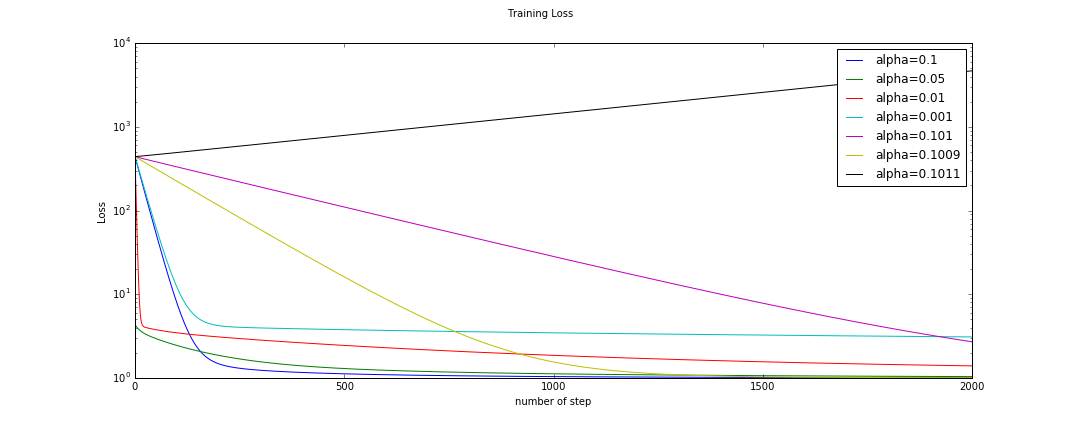
\includegraphics[width=\linewidth]{image242.png}
  \caption{Objective function for each step size.}
  \label{fig:242}
\end{figure}

{\bfseries Summary:}
From the Figure1, we can see, among the different step sizes alpha=0.05 converges most quickly and alpha=0.1 has the lowest loss. When step size equals 0.01 and 0.001, it seems that the objective function converges to local minimum instead of global minimum and maybe it is due to the step size is too small. when the alpha comes to 0.1009, though function still converges to global minimum, but the rate of converge is pretty slow. After step size bigger than 0.1011, instead of converging, the function seems to begin diverging.

        
\item (Optional, but recommended) Implement backtracking line search (google
it), and never have to worry choosing your step size again. How does
it compare to the best fixed step-size you found in terms of number
of steps? In terms of time? How does the extra time to run backtracking
line search at each step compare to the time it takes to compute the
gradient? (You can also compare the operation counts.)%2.4.3
\end{enumerate}

{\bfseries 2.4.3 Answer:}
\begin{lstlisting}
def BacktrackingLineSearch(func, df, x, p, args = (), alpha = 0.0001, beta = 0.9, eps = 1,):

    step_size = 1.0
    fc = 0
    len_p = norm(p)


    while func(x + step_size * p, args) > f_x + alpha * step_size * theta:
        step_size *= beta
        fc += 1
        if Verbose: print 'linesearch iteration', fc, ':', stp, f(x + stp * p, *args), f_x + alpha * stp * theta
        if stp * len_p < eps:
            print 'Step is  too small'
            break
    return step_size
    \end{lstlisting}

\subsection{Ridge Regression (i.e. Linear Regression with $L_{2}$ regularization)}%2.5

When we have a large number of features compared to instances, regularization
can help control overfitting. Ridge regression is linear regression
with $L_{2}$ regularization. The regularization term is sometimes
called a penalty term. The objective function for ridge regression
is
\[
J(\theta)=\frac{1}{2m}\sum_{i=1}^{m}\left(h_{\theta}(x_{i})-y_{i}\right)^{2}+\lambda\theta^{T}\theta,
\]
where $\lambda$ is the regularization parameter, which controls the
degree of regularization. Note that the bias parameter is being regularized
as well. We will address that below.
\begin{enumerate}
\item Compute the gradient of $J(\theta)$ and write down the expression%2.5.1
for updating $\theta$ in the gradient descent algorithm.

{\bfseries 2.5.1 Answer:}
$$\del_{\theta}J(\theta)=\frac{1}{m}X^{T}(X\theta-y)+ 2\lambda\theta$$
$$\theta:=\theta - \eta\del_{\theta}J(\theta)=\theta -\eta(\frac{1}{m}X^{T}(X\theta-y)+2\lambda\theta)$$


\item Implement \texttt{compute\_regularized\_square\_loss\_gradient.}%2.5.2

{\bfseries 2.5.2 Answer:}
\begin{lstlisting}
def compute_regularized_square_loss_gradient(X, y, theta, lambda_reg):
    """
    Compute the gradient of L2-regularized square loss function given X, y and theta
    
    Args:
        X - the feature vector, 2D numpy array of size (num_instances, num_features)
        y - the label vector, 1D numpy array of size (num_instances)
        theta - the parameter vector, 1D numpy array of size (num_features)
        lambda_reg - the regularization coefficient
    
    Returns:
        grad - gradient vector, 1D numpy array of size (num_features)
    """
    grad = compute_square_loss_gradient(X, y, theta)
    grad = grad + 2 * lambda_reg * theta
    return grad
            \end{lstlisting}



\item Implement \texttt{regularized\_grad\_descent.}%2.5.3

{\bfseries 2.5.3 Answer:}
\begin{lstlisting}
def regularized_grad_descent(X, y, alpha=0.01, lambda_reg=0.01, num_iter=1000):
    """
    Args:
        X - the feature vector, 2D numpy array of size (num_instances, num_features)
        y - the label vector, 1D numpy array of size (num_instances)
        alpha - step size in gradient descent
        lambda_reg - the regularization coefficient
        numIter - number of iterations to run 
        
    Returns:
        theta_hist - the history of parameter vector, 2D numpy array of size (num_iter+1, num_features) 
        loss_hist - the history of regularized loss value, 1D numpy array
    """
    (num_instances, num_features) = X.shape
    theta = np.ones(num_features) #Initialize theta
    theta_hist = np.zeros((num_iter+1, num_features))  #Initialize theta_hist
    loss_hist = np.zeros(num_iter+1) #Initialize loss_hist
    for i in range(num_iter):
        hypothesis = np.dot(X, theta)
        loss = hypothesis - y
        theta_hist[i] = theta
        loss_hist[i] = compute_square_loss(X, y, theta)
        gradient = compute_square_loss_gradient(X, y, theta)
        gradient = gradient + 2 * lambda_reg * theta
        theta = theta - alpha * gradient  # update
    theta_hist[i+1,:] = theta
    loss_hist[i+1] = compute_square_loss(X, y, theta) + ((2 *lambda_reg) / X.shape[0])*sum(theta**2)
    return theta_hist, loss_hist
                \end{lstlisting}



\item For regression problems, we may prefer to leave the bias term unregularized.
One approach is to change $J(\theta)$ so that the bias is separated
out from the other parameters and left unregularized. Another approach
that can achieve approximately the same thing is to use a very large
number $B$, rather than $1$, for the extra bias dimension. Explain
why making $B$ large decreases the effective regularization on the
bias term, and how we can make that regularization as weak as we like
(though not zero).%2.5.4

{\bfseries 2.5.4 Answer:}
$$J(\theta) = (\theta_{0}B+\theta_{1}x_{1}+.....+\theta_{n}x_{n})+\lambda\theta^{T}\theta$$
When B is a large number, to get the minimum loss, we have to set $\theta_{0}$ as small as possible, which means the regularization on bias term $\lambda\theta^{T}_{0}\theta_{0}$ is weak, since $\theta_{0}$ is tiny. Thus we can see, when making $B$ large,  the effective regularization on the bias term decreases.

\item (Optional) Develop a formal statement of the claim in the previous
problem, and prove the statement. 

{\bfseries 2.5.5 Answer:}
For regression problems, if B is a large number, then the regularization on bias term $\lambda\theta_{T}\theta$ is really small.
prove:
$$J(\theta) = (\theta_{0}B+\theta_{1}x_{1}+.....+\theta_{n}x_{n})+\lambda\theta^{T}\theta$$
Thus when $\lim_{B \to +\infty}$, to make $J(\theta)$ as small as possible, $\lim_{\theta _{0}\to 0}$.
So we can get
$$\lambda\theta^{T}_{0}\theta_{0}\to0$$
That is the regularization on this term is weak.

\item (Optional) Try various values of $B$ to see what performs best in
test.

\item Now fix $B=1$. Choosing a reasonable step-size (or using backtracking%2.5.7
line search), find the $\theta_{\lambda}^{*}$ that minimizes $J(\theta)$
over a range of $\lambda$. You should plot the training loss and
the test loss (just the square loss part, without the regularization,
in each case) as a function of $\lambda$. Your goal is to find $\lambda$
that gives the minimum test loss. It's hard to predict what $\lambda$
that will be, so you should start your search very broadly, looking
over several orders of magnitude. For example, $\lambda\in\left\{ 10^{-7},10^{-5},10^{-3},10^{-1},1,10,100\right\} $.
Once you find a range that works better, keep zooming in. You may
want to have $\log(\lambda)$ on the $x$-axis rather than $\lambda$.

{\bfseries 2.5.7 Answer:}

the minimum test loss is 1.220667675941963
the minimum train loss is 1.039074511634143

\begin{lstlisting}
lamb = np.linspace(1e-7, 0.1, 100)
plt.figure(figsize = (12, 6))
J_train = np.zeros(len(lamb))
J_test = np.zeros(len(lamb))
thetas = np.zeros((len(lamb),X_train.shape[1]))
axes = plt.gca()
for i in range(len(lamb)):
    theta, _ = regularized_grad_descent(X_train, y_train, alpha=0.1, lambda_reg = lamb[i], num_iter=1000)
    thetas[i] = theta[-1]
    J_train[i] = compute_square_loss(X_train, y_train, thetas[i])
    J_test[i] = compute_square_loss(X_test, y_test, thetas[i])
    
plt.plot(lamb, J_train, label = 'train_loss')
plt.plot(lamb, J_test, label = 'test_loss')
plt.xscale('log')
plt.xlabel('log(lambda)')
plt.ylabel('loss')
axes.set_ylim([0,10])
plt.legend()
                \end{lstlisting}
                
                
\begin{figure}
  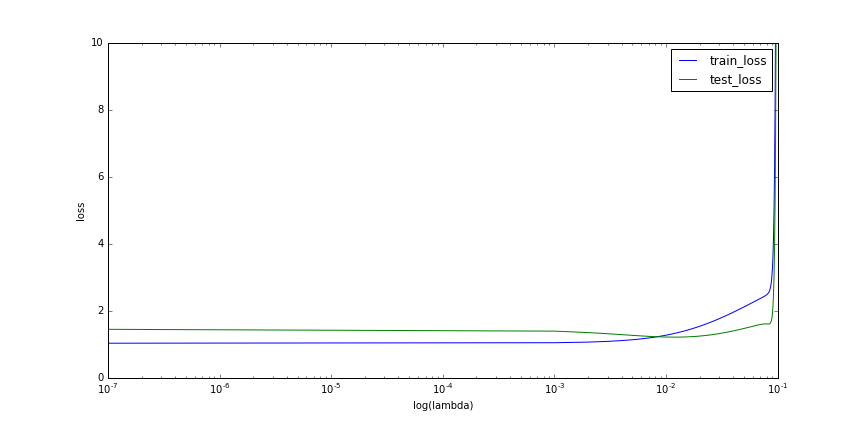
\includegraphics[width=\linewidth]{image257.png}
  \caption{Objective function for range of $\lambda$.}
  \label{fig:lambda}
\end{figure}

And the figure shows that when $\lambda$ is around 0.01, the function gives the minimum test loss.

\item What $\theta$ would you select for deployment and why?%2.5.8

{\bfseries 2.5.8 Answer:}
I would choose the $\theta$ trained by the lambda that gives the minimum test loss. Since the theta selected could gives the minimum loss on test set with the lambda we found, which is our goal.
\end{enumerate}

\subsection{Stochastic Gradient Descent}

\noindent When the training data set is very large, evaluating the
gradient of the loss function can take a long time, since it requires
looking at each training example to take a single gradient step. In
this case, stochastic gradient descent (SGD) can be very effective.
In SGD, the gradient of the risk is approximated by a gradient at
a single example. The approximation is poor, but it is unbiased. The
algorithm sweeps through the whole training set one by one, and performs
an update for each training example individually. One pass through
the data is called an \emph{epoch}. Note that each epoch of SGD touches
as much data as a single step of batch gradient descent. Before we
begin cycling through the training examples, it is important to shuffle
the examples into a random order. You can use the same ordering for
each epoch, though optionally you could investigate whether reshuffling%2.6
after each epoch speeds up convergence. 
\begin{enumerate}
\item \emph{W}rite down the update rule for $\theta$ in SGD for the ridge
regression objective function.%2.6.1

{\bfseries 2.6.1 Answer:}
$$\theta_{t+1}:=\theta_{t} - \eta\del_{\theta_{t}}J(\theta_{t})=\theta_{t} -\eta(\frac{1}{m}X^{T}(x_{i}\theta_{t}-y_{i})+2\lambda\theta_{t})$$

\item Implement \texttt{stochastic\_grad\_descent}. (Note: You could potentially
reuse the code you wrote for batch gradient, though this is not necessary.
If we were doing minibatch gradient descent with batch size greater
than 1, you would definitely want to use the same code.)%2.6.2

{\bfseries 2.6.2 Answer:}
\begin{lstlisting}
import random
import timeit
def stochastic_grad_descent(X, y, alpha=0.1, lambda_reg=1, num_iter=1000):
    """
    In this question you will implement stochastic gradient descent with a regularization term
    
    Args:
        X - the feature vector, 2D numpy array of size (num_instances, num_features)
        y - the label vector, 1D numpy array of size (num_instances)
        alpha - string or float. step size in gradient descent
                NOTE: In SGD, it's not always a good idea to use a fixed step size. Usually it's set to 1/sqrt(t) or 1/t
                if alpha is a float, then the step size in every iteration is alpha.
                if alpha == "1/sqrt(t)", alpha = 1/sqrt(t)
                if alpha == "1/t", alpha = 1/t
        lambda_reg - the regularization coefficient
        num_iter - number of epochs (i.e number of times) to go through the whole training set
    
    Returns:
        theta_hist - the history of parameter vector, 3D numpy array of size (num_iter, num_instances, num_features) 
        loss hist - the history of regularized loss function vector, 2D numpy array of size(num_iter, num_instances)
        time - the amount of time it takes on your computer for a single epoch of SGD
    """
    num_instances, num_features = X.shape[0], X.shape[1]
    theta = np.ones(num_features) #Initialize theta
    theta_hist = np.zeros((num_iter, num_instances, num_features))  #Initialize theta_hist
    loss_hist = np.zeros((num_iter, num_instances)) #Initialize loss_hist
    batchsize = num_instances / num_iter
    time = []
    n = list(range(num_instances))
    for epoch in np.arange(0, num_iter):
        #epoch_loss = []
        np.random.shuffle(n)
        start = timeit.default_timer()
        for i in range(len(n)):
            loss = 0
            if type(alpha) == float:
                eta = alpha
            elif alpha == "1/sqrt(t)":
                eta = 0.1 / np.sqrt(i+1)
            else:
                eta = 0.1/(i+1)
            hypothesis = np.sum(X[n[i]] * theta)
            loss = hypothesis - y[n[i]]
            cost = loss*loss
            gradient = np.dot(X[n[i]], loss)
            gradient = gradient + 2 * lambda_reg * theta
            theta = theta - eta * gradient
            theta_hist[epoch,i] = theta
            loss_hist[epoch,n[i]] = cost
        stop = timeit.default_timer()
        time.append(stop - start)
    return theta_hist, loss_hist, time                
    \end{lstlisting}


\item Use SGD to find $\theta_{\lambda}^{*}$ that minimizes the ridge regression
objective for the $\lambda$ and $B$ that you selected in the previous
problem. (If you could not solve the previous problem, choose $\lambda=10^{-2}$
and $B=1$). Try a few fixed step sizes (at least try $\eta_{t}\in\left\{ 0.05,.005\right\} $.
Note that SGD may not converge with fixed step size. Simply note your
results. Next try step sizes that decrease with the step number according
to the following schedules: $\eta_{t}=\frac{1}{t}$ and $\eta_{t}=\frac{1}{\sqrt{t}}$.
For each step size rule, plot the value of the objective function
(or the log of the objective function if that is more clear) as a
function of epoch (or step number) for each of the approaches to step
size. How do the results compare? Two things to note: 1) In this case
we are investigating the convergence rate of the optimization algorithm
with different step size schedules, thus we're interested in the value
of the objective function, which includes the regularization term.
2) As we'll learn in an upcoming lecture, SGD convergence is much
slower than GD once we get close to the minimizer. (Remember, the
SGD step directions are very noisy versions of the GD step direction).
If you look at the objective function values on a logarithmic scale,
it may look like SGD will never find objective values that are as
low as GD gets. In terms we'll discuss in Week 2, GD has much smaller
``optimization error'' than SGD. However, this difference in optimization
error is usually dominated by other sources of error (estimation error
and approximation error, which we'll also discuss in Week 2). Moreover,
for very large datasets, SGD (or minibatch GD) is much faster (by
wall-clock time) than GD to reach a point that's close enough to the
minimum. %2.6.3

{\bfseries 2.6.2 Answer:}
\begin{lstlisting}
import timeit

alpha = [0.05,0.005,0.01,0.001]
fig = plt.figure(figsize = (12,6))
axes = plt.gca()

for i in range(len(alpha)):
    theta, loss, time = stochastic_grad_descent(X_train, y_train, alpha='y', lambda_reg=0.01, num_iter=100)
    plt.plot(np.arange(0, 100),loss, label = alpha[i])

fig.suptitle("Training Loss")
plt.xlabel("Epoch #")
plt.ylabel("Loss")
axes.set_ylim([0,10])
plt.legend()
                \end{lstlisting}
         
\begin{lstlisting}
import timeit

alpha = [0.05,0.005,0.01,0.001]
fig = plt.figure(figsize = (12,6))
axes = plt.gca()

for i in range(len(alpha)):
    theta, loss, time = stochastic_grad_descent(X_train, y_train, alpha='y', lambda_reg=0.01, num_iter=100)
    plt.plot(np.arange(0, 100),loss, label = alpha[i])

fig.suptitle("Training Loss")
plt.xlabel("Epoch #")
plt.ylabel("Loss")
axes.set_ylim([0,10])
plt.legend()
                \end{lstlisting}

\begin{figure}
  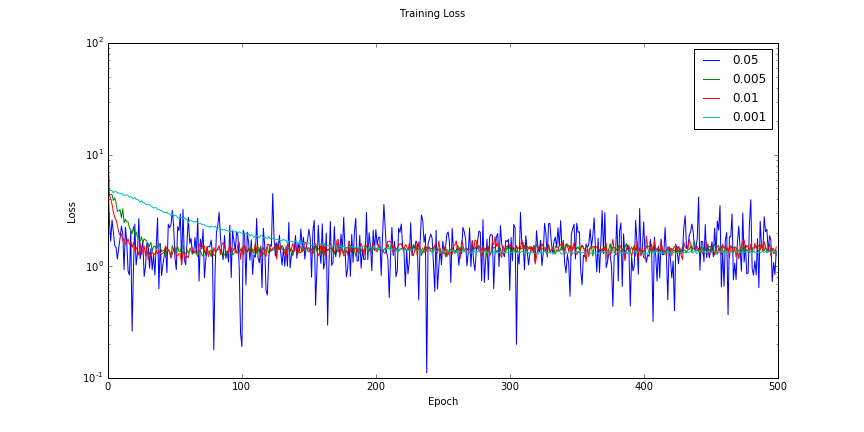
\includegraphics[width=\linewidth]{image2631.png}
  \caption{Objective function for fixed step sizes.}
  \label{fig:sgd1}
\end{figure} 

\begin{figure}
  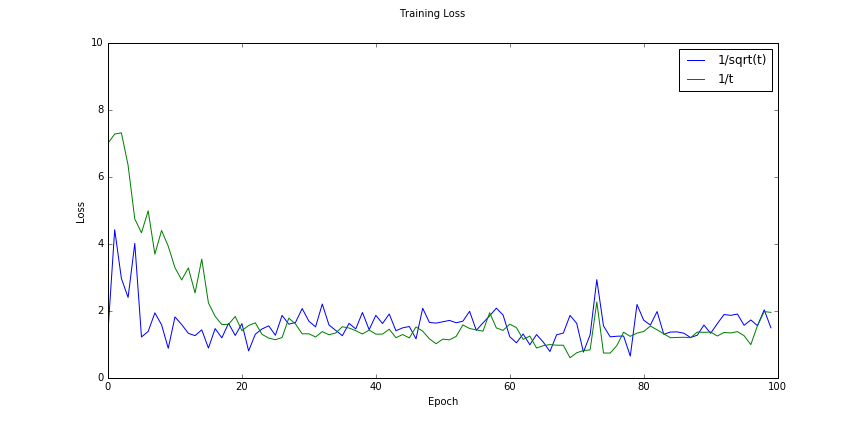
\includegraphics[width=\linewidth]{image2632.png}
  \caption{Objective function for updating step sizes.}
  \label{fig:sgd2}
\end{figure}        

   
         
                
\item Estimate the amount of time it takes on your computer for a single
epoch of SGD. %2.6.4

{\bfseries 2.6.4 Answer:}
The average time it takes on my computer for a single epoch of SGD is 0.0031s.
The maximum time it takes on my computer for a single epoch of SGD is 0.0048s.
The minimum time it takes on my computer for a single epoch of SGD is 0.0027s.


\item Comparing SGD and gradient descent, if your goal is to minimize the
total number of epochs (for SGD) or steps (for batch gradient descent),
which would you choose? If your goal were to minimize the total time,
which would you choose?%2.6.5

{\bfseries 2.6.5 Answer:}
If my goal is to minimize the total number of epochs or steps, I would choose the gradient descent.
If my goal is to minimize the total time, I would choose the SGD. SGD will be faster because you use only one training sample and it starts improving itself right away from the first sample.
\end{enumerate}

\section{Risk Minimization}%3

\subsection{Square Loss}%3.1

\global\long\def\E{\ex}

\begin{enumerate}
\item Let $y$ be a random variable with a known distribution, and consider
the square loss function $\ell(a,y)=(a-y)^{2}$. We want to find the
action $a^{*}$ that has minimal risk. That is, we want to find $a^{*}=\argmin_{a}\ex\left(a-y\right)^{2}$,
where the expectation is with respect to $y$. Show that $a^{*}=\ex y$,
and the Bayes risk (i.e. the risk of $a^{*}$) is $\var(y)$. In other
words, if you want to try to predict the value of a random variable
drawn, the best you can do (for minimizing square loss) is to predict
the mean of the distribution. Your expected loss for predicting the
mean will be the variance of the distribution. {[}Hint: Recall that
$\var(y)=\ex y^{2}-\left(\ex y\right)^{2}$.{]}%3.1

{\bfseries 3.1.1 Answer:}
%$$R(a^{*}) = \ex\left(a^{*}-y\right)^{2}$$

\begin{align}
R(a) = \ex[\left(a-y\right)^{2}]
=& \ex[(a-\ex[y]+\ex[y]-y)^{2}]\\
=& \ex[(a-\ex[y])^{2}]+\ex[\ex[y]-y)^{2}]+\ex[2(a-\ex[y])(\ex[y]-y)]\\
=& \ex[(a-\ex[y])^{2}]+\ex[\ex[y]-y)^{2}]+2\ex[(a-\ex[y])(\ex[y]-y)]\\
\end{align}
Since $\ex[y]-a$ and $\ex[y]$ are const, we can get:
\begin{align}
R(a)= \ex[\left(a-y\right)^{2}]
=& \ex[(a-\ex[y])^{2}]+(\ex[y]-y)^{2}+2(a-\ex[y])(\ex[y]-\ex[y]))\\
=& \ex[(a-\ex[y])^{2}]+\ex[(\ex[y]-y)^{2}]\\
=& Var(y)+\left(\ex[y]-a\right)^{2}\\
\end{align}
To make the loss function$R(a)$ get the minimum value, $a$ should equal to $\ex[y]$, so that $\left(\ex[y]-a\right)^{2}=0$

Thus, $R(a^{*})=Var(y)+\left(\ex[y]-a^{*}\right)^{2} = Var(y)$

Which is the Bayes Risk.

\item Now let's introduce an input. Recall that the \textbf{expected loss
}or \textbf{``risk''}\emph{ }of a decision function $f:\cx\to\ca$
is
\[
R(f)=\ex\loss(f(x),y),
\]
where $(x,y)\sim P_{\cx\times\cy}$, and the \textbf{Bayes decision
function} $f^{*}:\cx\to\ca$ is a function that achieves the \emph{minimal
risk} among all possible functions: 
\[
R(f^{*})=\inf_{f}R(f).
\]
Here we consider the regression setting, in which $\ca=\cy=\reals$.
We will show for the square loss $\ell(a,y)=\left(a-y\right)^{2}$,
the Bayes decision function is $f^{*}(x)=\ex\left[y\mid x\right]$,
where the expectation is over $y$. As before, we assume know the
data-generating distribution $P_{\cx\times\cy}$.
\begin{enumerate}
\item We'll approach this problem by finding the optimal action for any
given $x$. If somebody tells us $x$, we know that the corresponding
$y$ is coming from the conditional distribution $y\mid x$. For a
particular $x$, what value should we predict (i.e. what action $a$
should we produce) that has minimal expected loss? Express your answer
as a decision function $f(x)$, which gives the best action for any
given $x$. In mathematical notation, we're looking for $f^{*}(x)=\argmin_{a}\ex\left[\left(a-y\right)^{2}\mid x\right]$,
where the expectation is with respect to $y$.%3.2

{\bfseries 3.1.2 (a) Answer:}
$$f^{*}=\ex[y|x]$$
{\bfseries prove:}
\begin{align}
R(f) = \ex[\left(f(x)-y\right)^{2}]
=& \ex[(f(x)-\ex[y|x]+\ex[y|x]-y)^{2}]\\
=& \ex[(f(x)-\ex[y|x])^{2}]+\ex[\ex[y|x]-y)^{2}]+2\ex[(f(x)-\ex[y|x])(\ex[y|x]-y)]\\
=& \ex[(f(x)-\ex[y|x])^{2}]+\ex[\ex[y|x]-y)^{2}]+2\ex[(f(x)-\ex[y|x])\ex[(\ex[y|x]-y)|x]]\\
=& \ex[(f(x)-\ex[y|x])^{2}]+\ex[\ex[y|x]-y)^{2}]+2\ex[(f(x)-\ex[y|x])(\ex[y|x]-\ex[y|x]]\\
=& \ex[(f(x)-\ex[y|x])^{2}]+\ex[\ex[y|x]-y)^{2}]\\
=& \ex[(f(x)-\ex[y|x])^{2}]+\ex[Var(y)]
\end{align}
Since $\ex[Var(y)]$ is independent of y, thus taking $f^{*}=\ex[y|x]$ minimizes the expected loss.


\item In the previous problem we produced a decision function $f^{*}(x)$
that minimized the risk for each $x$. In other words, for any other
decision function $f(x)$, $f^{*}(x)$ is going to be at least as
good as $f(x)$, for every single $x$. That is
\[
\ex\left[\left(f^{*}(x)-y\right)^{2}\mid x\right]\le\ex\left[\left(f(x)-y\right)^{2}\mid x\right],
\]
for all $x$. To show that $f^{*}(x)$ is the Bayes decision function,
we need to show that 
\[
\ex\left[\left(f^{*}(x)-y\right)^{2}\right]\le\ex\left[\left(f(x)-y\right)^{2}\right]
\]
for any $f$. Explain why this is true.

{\bfseries 3.1.2 (b) Answer:}
$$\ex\left[\left(f(x)-y\right)^{2}\right]=\int(f(x)-\ex[y|x])^{2}p(x)dx+\int(\ex[y|x]-y)^{2}p(x)dx$$
\begin{align}
\ex\left[\left(f(x^{*})-y\right)^{2}\right]
=&\int(f^{*}(x)-\ex[y|x])^{2}p(x)dx+\int(\ex[y|x]-y)^{2}p(x)dx\\
=&\int(\ex[y|x]-\ex[y|x])^{2}p(x)dx+\int(\ex[y|x]-y)^{2}p(x)dx\\
=&\int(\ex[y|x]-y)^{2}p(x)dx\\
<=& \int(f(x)-\ex[y|x])^{2}p(x)dx+\int(\ex[y|x]-y)^{2}p(x)dx\\
=& \ex\left[\left(f(x)-y\right)^{2}\right]\\
\end{align}
Thus 
\[
\ex\left[\left(f^{*}(x)-y\right)^{2}\right]\le\ex\left[\left(f(x)-y\right)^{2}\right]
\]
of any $f$ is true.
\end{enumerate}
\end{enumerate}

\subsection{{[}Optional{]} Median Loss}
\begin{enumerate}
\item (Optional) Show that for the absolute loss $\ell(\hat{y},y)=\left|y-\hat{y}\right|$,
then $f^{*}(x)$ is a Bayes decision function iff $f^{*}(x)$ is the
median of the conditional distribution of $y$ given $x$. {[}Hint:
As in the previous section, consider one $x$ at time. It may help
to use the following characterization of a median: $m$ is a median
of the distribution for random variable $Y$ if $P(Y\ge m)\ge\frac{1}{2}$
and $P(Y\le m)\ge\frac{1}{2}$.{]} Note: This loss function leads
to ``median regression''. There are other loss functions that lead
to ``quantile regression'' for any chosen quantile. 
\end{enumerate}

\end{document}
